\documentclass[12pt,twoside]{report}
\usepackage[utf8]{inputenc}
\usepackage{graphicx}
\usepackage[colorlinks=true,linkcolor=black,anchorcolor=black,citecolor=black,filecolor=black,menucolor=black,runcolor=black,urlcolor=black]{hyperref}
\usepackage[a4paper,width=150mm,top=25mm,bottom=25mm,bindingoffset=6mm]{geometry}
\usepackage{fancyhdr}
\usepackage{caption}
\usepackage{subcaption}
\renewcommand{\headrulewidth}{0.4pt}
\renewcommand{\footrulewidth}{0.4pt}
\setlength{\headheight}{27.5pt}
\pagestyle{fancy}
\graphicspath{ {images/} }
\title{
{Designing and implementing an smart monitoring and management system of environmental and electrical conditions of server rooms
    }\\
    {
\includegraphics{logo.jpg}}\\
    {\large University of Guilan}

}
\author{
  Mokadar Daemdoost, Amin\\
  \texttt{amindaemdoost@yahoo.com}
  \and
  Abbasi, Poorya\\
  \texttt{hey@pooryaa.com}
}
\date{30 Jan 2023}

\begin{document}
\fancyhead{}
\fancyhead[RO,LE]{Designing and implementing an smart monitoring and management system of environmental and electrical conditions of server rooms}
\fancyfoot{}
\fancyfoot[LE,RO]{\thepage}
\fancyfoot[LO,RE]{Chapter \thechapter}
\fancyfoot[CO,CE]{A. Mokadar Daemdoost, P. Abbasi}
    \maketitle
    \begin{abstract}
      The design and implementation of a server room monitoring system, which tracks significant environmental factors like temperature, humidity, and dust levels, are presented in this thesis. The system is made to give real-time updates on the circumstances in the server room, ensuring that the servers and other equipment are working properly.\\
In order to retrieve data from the database and return it in a format that the front-end can use, Node.js was used to build a REST API for the back-end. We used Prisma and PostgreSQL to provide the necessary data management and storage features. The efficient and scalable handling of massive amounts of data is ensured by the use of Node.js, Prisma, and PostgreSQL, and the type-safe API offered by Prisma makes it simpler to retrieve and manipulate the data.
\\
An interface that provides real-time updates on the circumstances in the server room was made for the front-end using React, Next.js, and Tailwind. While Next.js offers server-side rendering and enhanced performance, React offers a robust and adaptable framework for creating user interfaces. Rapid and effective front-end development is made possible by Tailwind's selection of pre-made UI elements and styling tools.
    \end{abstract}
    \tableofcontents

    \chapter{Introduction}
    
\section{Backgrounds}
    Server rooms are a critical component of today's technology-driven world: with the growing reliance on and need for technological devices, ensuring that server rooms function properly has become an essential part of our daily lives. Server rooms are important to an organization because they contain infrastructure and critical equipment. Monitoring various parameters such as temperature, humidity, electricity and others helps ensure that the system is running smoothly. The first step in monitoring server rooms is to understand the different parameters that need to be monitored. The following is a list of common parameters that should be monitored in server rooms :\\
    \begin{itemize}
        \item Temperature
            \begin{description}
                \item Server room temperature should be maintained at a stable, suitable level to ensure the proper functioning of equipment. The recommended range of temperatures is between 18°C and 27°C.  \cite{ASHRAE_Storage_White_Paper_2015}
                \begin{description}
                    \item[Too high temperature:] If the temperature inside a server room rises above the recommended range, it can cause several problems. High temperatures can make equipment operate less efficiently and potentially fail altogether. High temperatures can also decrease the life expectancy of electronic devices and increase the chance that stored data will be corrupted. \cite{data_center_cooling}
                    \item[Too low temperature:] If the temperature in a server room is allowed to fall below the recommended range, it can cause several issues. The cold air can lead to condensation—which leads directly to corrosion and equipment damage. In addition, low temperatures can decrease the efficiency of equipment and make it more likely to fail. \cite{data_center_cooling}
                \end{description}
            \end{description}
        \item Humidity
            \begin{description}
                \item On the other hand, High humidity levels can lead to condensation, which causes corrosion of the equipment and short circuits. High humidity levels can also create conditions that are conducive to the growth of mold and other microorganisms, which in turn damage equipment and affect indoor air quality. \cite{10.1115/IPACK2015-48176}
            \end{description}
        \item Dust
            \begin{description}
                \item Dust accumulation in a server room can degrade the performance and lifespan of equipment. Dust can block air vents, causing overheating, and it also attracts moisture leading to corrosion or other problems. So monitoring the levels of dust in a server room can help identifying and addressing potential problems.
            \end{description}
        \item Water Leakage
            \begin{description}
                \item Serious consequences can result from water leakage in a server room, even if only a small amount of water leaks onto equipment. It is important to have proper monitoring systems and alerts that will notify personnel as soon as possible after any leak occurs. \cite{telecommunications2010tia}
            \end{description}
        \item Electricity
            \begin{description}
                \item Monitoring the state of electricity, including voltage and current, is important in a server room to ensure the stability and reliability of the power supply to the equipment. Electrical voltage and current fluctuations can lead to problems with electronic equipment, such as data loss and corruption. In order to minimize these risks, server rooms are typically equipped with uninterruptible power supplies (UPS) and surge protection devices that help stabilize the voltage. The following list contains some common ranges for voltage and current.\cite{telecommunications2010tia}
                \begin{description}
                    \item[Voltage:] The recommended operating range in from 208V to 240V and the maximum recommended limit is 264V.
                    \item[Current:] The recommended operating range in from 20A to 40A (per phase)
                \end{description}
            \end{description}
        \item Movement
            \begin{description}
                \item Movement sensors, also known as motion detectors, can be used in order to detect unauthorized access to the room by detecting movements within the room and alerting the administrators.
                \begin{description}
                    \item[Voltage:] The recommended operating range in from 208V to 240V and the maximum recommended limit is 264V.
                    \item[Current:] The recommended operating range in from 20A to 40A (per phase)
                \end{description}
            \end{description}
        \end{itemize}

        \section{Purpose}
            The purpose of this thesis is to demonstrate how an effective and efficient monitoring system can be implemented for server rooms using sensors, which are introduced in three categories in the tables \ref{table:electrical_sensors}, \ref{table:envirement_sen} and \ref{table:security_sen}. The system will be designed to provide real-time data to a website, so that it can be monitored anywhere with internet access. This thesis will examine how this system was designed and implemented, including the selection of sensors and development of an online panel for monitoring data visualization.
            
            \begin{table}
                \centering
                \caption{Electrical sensors}
                \begin{tabular}{ |c|c|c|c|c|c|}
                \hline
                {\textbf{Name}} & {\textbf{Measurement Unit}} & {\textbf{Output}} \\ 
                \hline

                Voltage Sensor & Voltage &  ADC \\
                \hline
                
                Current Sensor & Amper &  ADC \\
                \hline
                \end{tabular}
                \label {table:electrical_sensors}
            \end{table}
               
            \begin{table}
                \centering
                \caption{Environment sensors}
                \begin{tabular}{ |c|c|c|c|c|c|}
                    \hline
                    {\textbf{Name}} & {\textbf{Measurement Unit}} & {\textbf{Operating temp}}& {\textbf{Desired values}}   \\ 
                    \hline

                    Temperature sensor & Celsius & -20°C - 50°C & 18°C - 27°C\\
                    \hline
                    Smoke sensor &  - & -20°C - 50°C & -  \\
                    \hline
                    Humidity sensor & Percent &  -20°C - 50°C & 40\% - 60\% \\
                    \hline
                    Water Leakage Sensor &  - & -20°C - 50°C & -  \\
                    \hline
                    Dust sensor &  - & -20°C - 50°C & -  \\
                    \hline
                \end{tabular}
                \label {table:envirement_sen}
            \end{table}
        
            \begin{table}
                \centering
                \caption{Security sensors}
                \begin{tabular}{ |c|c|c|c|c|c|}
                    \hline
                    {\textbf{Name}}  \\ 
                    \hline

                    Movement sensor  \\
                    \hline
                    Fingerprint sensor  \\
                    \hline
                    Camera \\
                    \hline
                \end{tabular}
                \label{table:security_sen}
            \end{table}
          




    \chapter{Data Generator Selection and Implementation}
    \section{Introduction}
    In this implementation, in order to demonstrate how the monitoring system works instead of using actual sensors, a data generator has been used and it simulates reading of sensors (such as humidity, temperature and electricity).

\section{Methodology}
A data generator should have a random yet realistic pattern for effective system testing, so just using a simple random number would be insufficient. Therefore, in this thesis a controlled version of choosing a random number was used to mimic some parts of real-world criteria and avoid sudden changes. The methodology for this process can be seen in the accompanying flowchart \ref{chart:data_gen}.\\


    \begin{figure}
        \centering
        \captionsetup{type=figure}
        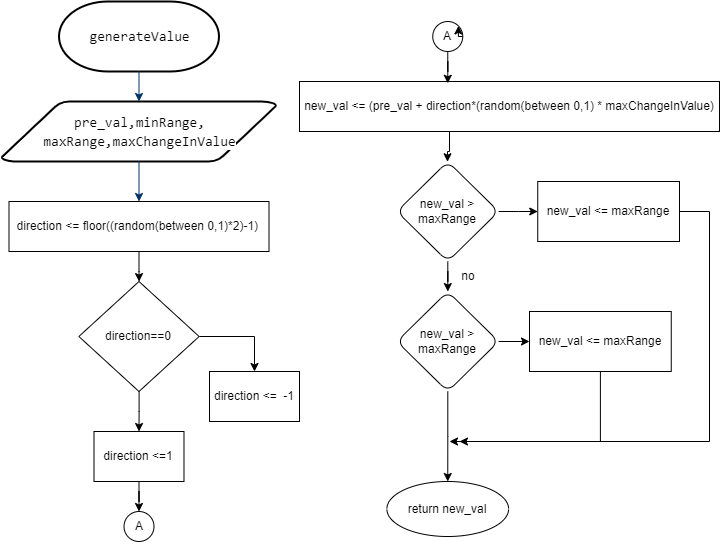
\includegraphics[width=1\textwidth]{flowchart_data_gen}
        \caption{Flowchart of data generator}
        \label{chart:data_gen}
    \end{figure}

\section{Results}
    As discussed in the methodology section, the program was implemented, and the generated values tested with different parameters was saved and reported as line charts in the subsequent sections.
    \subsection{Generated temperature sensor data}
        \begin{itemize}
            \item Parameters
                \begin{description}
                    \item[Starting Temperature sensor Value:] 22
                    \item[Minimum Possible Temperature sensor value:] 18
                    \item[Maximum Possible Temperature sensor value:] 27
                    \item[Maximum Possible Change in an iteration:] 0.5
                \end{description}
            \item Results can be seen in figure \ref{fig:gen_temperature}
                \begin{figure}
                    \centering
                    \captionsetup{type=figure}
                    \begin{subfigure}[b]{0.45\textwidth}
                        \centering
                        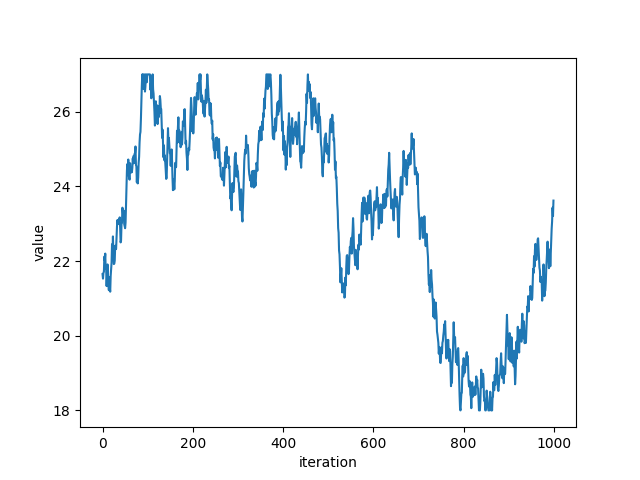
\includegraphics[width=\textwidth]{linechart_data_gen_temperature1000i}
                        \caption{For 1000 iterations}
                        \label{chart:gen_temperature_1000}
                    \end{subfigure}
                    \hfill
                    \begin{subfigure}[b]{0.45\textwidth}
                        \centering
                        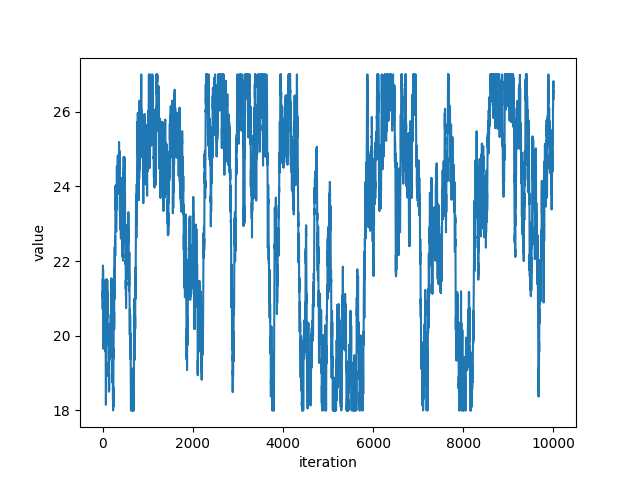
\includegraphics[width=\textwidth]{linechart_data_gen_temperature10000i}
                        \caption{For 10000 iterations}
                        \label{chart:gen_temperature_10000}
                    \end{subfigure}
                    
                    \caption{Sample generated temperature sensor data }
                    \label{fig:gen_temperature}
                \end{figure}
            \end{itemize}
            \subsection{Generated humidity sensor data}
                \begin{itemize}
                    \item Parameters
                        \begin{description}
                            \item[Starting humidity sensor value:] 55
                            \item[Minimum possible humidity sensor value:] 40
                            \item[Maximum possible humidity:] 60
                            \item[Maximum possible Change in an iteration:] 0.5
                        \end{description}
                    \item Results can be seen in figure \ref{fig:gen_humidity}
                        \begin{figure}
                            \centering
                            \captionsetup{type=figure}
                            \begin{subfigure}[b]{0.45\textwidth}
                                \centering
                                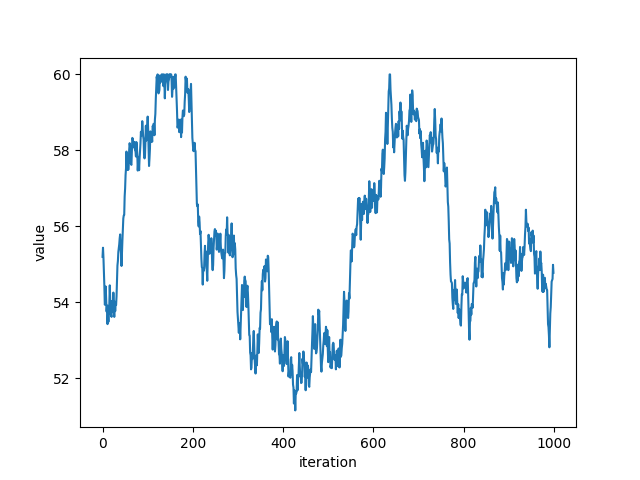
\includegraphics[width=\textwidth]{linechart_data_gen_humidity1000i}
                                \caption{For 1000 iterations}
                                \label{chart:gen_humidity_1000}
                            \end{subfigure}
                            \hfill
                            \begin{subfigure}[b]{0.45\textwidth}
                                \centering
                                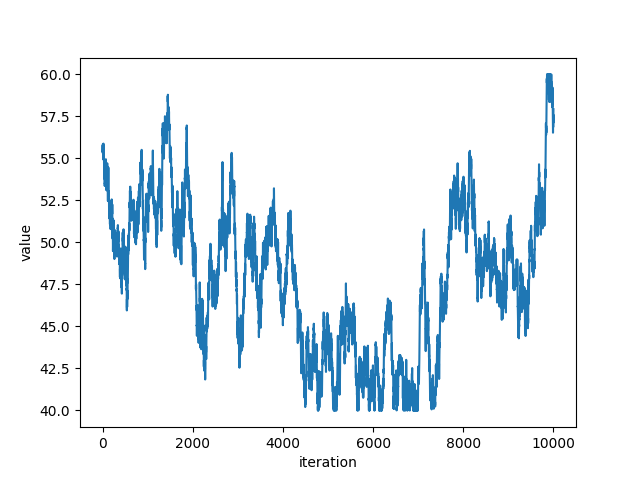
\includegraphics[width=\textwidth]{linechart_data_gen_humidity10000i}
                                \caption{For 10000 iterations}
                                \label{chart:gen_humidity_10000}
                            \end{subfigure}
                            
                            \caption{Sample generated humidity sensor data }
                            \label{fig:gen_humidity}
                        \end{figure}
                    \end{itemize}
                \subsection{Generated dust sensor data}
                    \begin{itemize}
                        \item Parameters
                            \begin{description}
                                \item[Starting dust sensor Value:] 1
                                \item[Minimum possible dust sensor value:] 0
                                \item[Maximum possible dust sensor value:] 3
                                \item[Maximum possible change in an iteration:] 0.5
                            \end{description}
                        \item Results can be seen in figure \ref{fig:gen_dust}
                            \begin{figure}
                                \centering
                                \captionsetup{type=figure}
                                \begin{subfigure}[b]{0.45\textwidth}
                                    \centering
                                    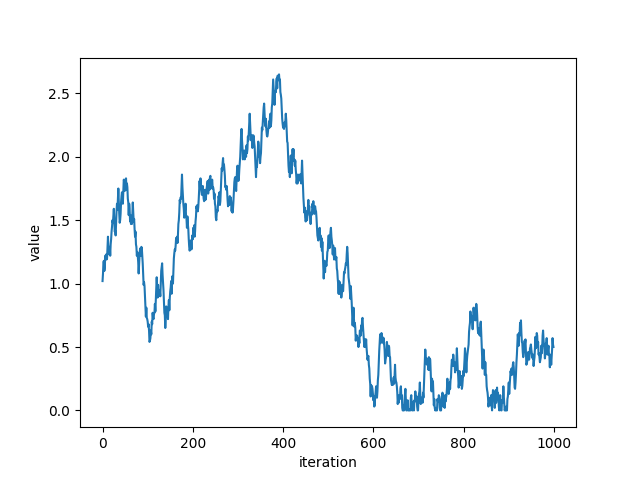
\includegraphics[width=\textwidth]{linechart_data_gen_dust1000i}
                                    \caption{For 1000 iterations}
                                    \label{chart:gen_dust_1000}
                                \end{subfigure}
                                \hfill
                                \begin{subfigure}[b]{0.45\textwidth}
                                    \centering
                                    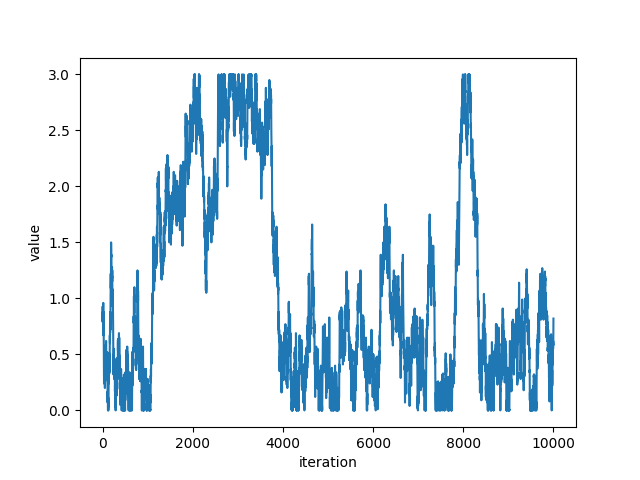
\includegraphics[width=\textwidth]{linechart_data_gen_dust10000i}
                                    \caption{For 10000 iterations}
                                    \label{chart:gen_dust_10000}
                                \end{subfigure}
                                
                                \caption{Sample generated dust sensor data }
                                \label{fig:gen_dust}
                        \end{figure}
                    \end{itemize}
                \subsection{Generated electricity voltage sensor data}
                        \begin{itemize}
                            \item Parameters
                                \begin{description}
                                    \item[Starting electricity voltage value:] 220
                                    \item[Minimum possible electricity voltage:] 208
                                    \item[Maximum possible electricity voltage:] 264
                                    \item[Maximum possible electricity change in an iteration:] 1
                                \end{description}
                            \item Results can be seen in figure \ref{fig:gen_voltage}
                                \begin{figure}
                                    \centering
                                    \captionsetup{type=figure}
                                    \begin{subfigure}[b]{0.45\textwidth}
                                        \centering
                                        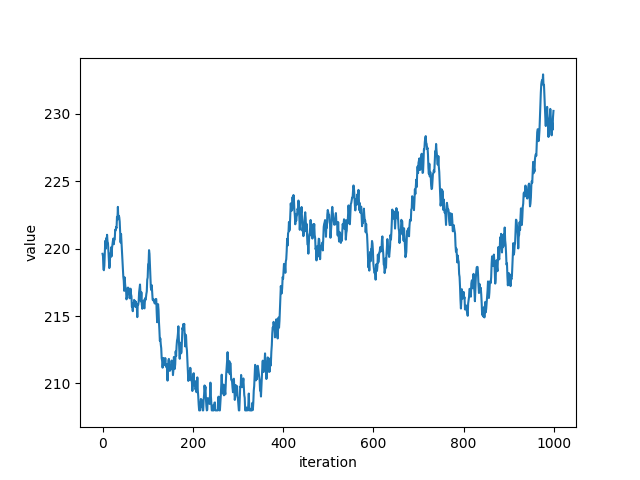
\includegraphics[width=\textwidth]{linechart_data_gen_voltage1000i}
                                        \caption{For 1000 iterations}
                                        \label{chart:gen_voltage_1000}
                                    \end{subfigure}
                                    \hfill
                                    \begin{subfigure}[b]{0.45\textwidth}
                                        \centering
                                        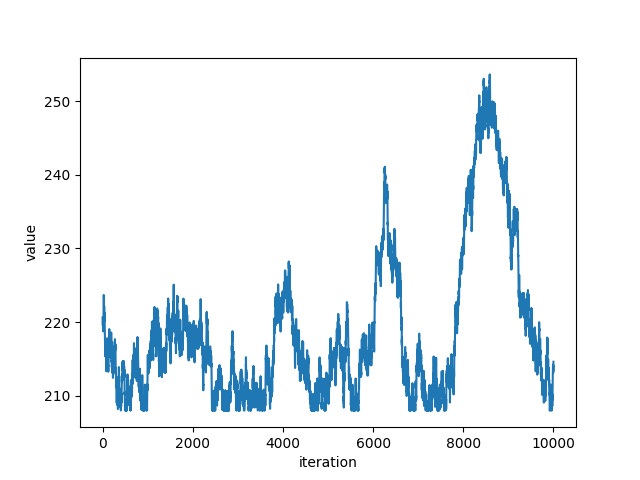
\includegraphics[width=\textwidth]{linechart_data_gen_voltage10000i}
                                        \caption{For 10000 iterations}
                                        \label{chart:gen_voltage_10000}
                                    \end{subfigure}
                                    
                                    \caption{Sample generated voltage sensor data }
                                    \label{fig:gen_voltage}
                            \end{figure}
                        \end{itemize}


                    \subsection{Generated electricity current sensor data}
                        \begin{itemize}
                            \item Parameters
                                \begin{description}
                                    \item[Starting electricity Current Value:] 30
                                    \item[Minimum possible electricity Current:] 20
                                    \item[Maximum possible electricity Current:] 40
                                    \item[Maximum possible change in an iteration:] 1
                                \end{description}
                            \item Results can be seen in figure \ref{fig:gen_current}
                                \begin{figure}
                                    \centering
                                    \captionsetup{type=figure}
                                    \begin{subfigure}[b]{0.45\textwidth}
                                        \centering
                                        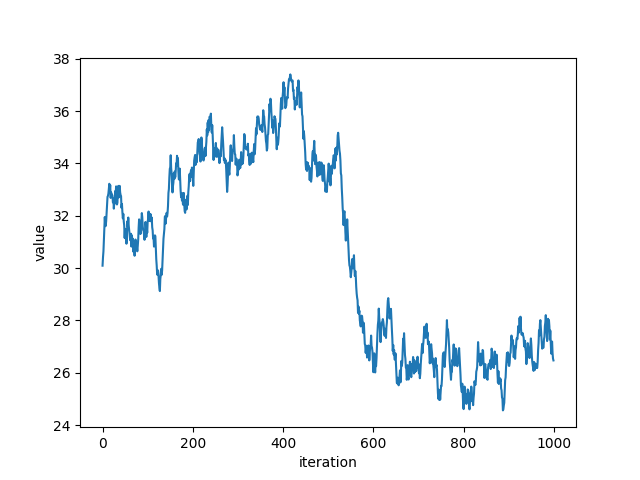
\includegraphics[width=\textwidth]{linechart_data_gen_current1000i}
                                        \caption{For 1000 iterations}
                                        \label{chart:gen_current_1000}
                                    \end{subfigure}
                                    \hfill
                                    \begin{subfigure}[b]{0.45\textwidth}
                                        \centering
                                        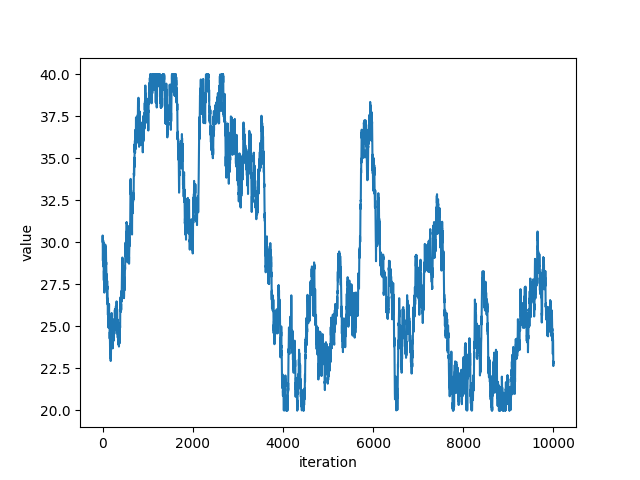
\includegraphics[width=\textwidth]{linechart_data_gen_current10000i}
                                        \caption{For 10000 iterations}
                                        \label{chart:gen_current_10000}
                                    \end{subfigure}
                                    
                                    \caption{Sample generated voltage sensor data }
                                    \label{fig:gen_current}
                            \end{figure}
                        \end{itemize}
        


    \chapter{Panel Design and Implementation}
    \section{Introduction}
A good server room monitoring system panel is an essential component for ensuring the proper functioning of a server room environment. It provides real-time monitoring of key physical and environmental factors such as temperature, humidity, power, and network connectivity. The panel alerts administrators in case of any deviations from the defined thresholds, helping prevent potential data loss, hardware damage, and downtime. Additionally, a good server room monitoring system panel provides historical data and reporting capabilities, allowing administrators to track trends and make informed decisions about capacity planning and infrastructure improvements. With the right server room monitoring system panel in place, organizations can ensure the safety and reliability of their critical IT assets.
\section{Back-end}
Node.js, PostgreSQL, and Prisma can be used together to build a robust and scalable back-end for a server room monitoring panel.
    \subsection{Node js} 
    Node.js is a JavaScript runtime built on Chrome's V8 JavaScript engine, and is a critical component in building a server room monitoring panel's back-end. Node.js allows developers to use JavaScript on the server-side, providing a unified language for both client-side and server-side development. This helps to simplify the development process and increase developer productivity.\\
    In a server room monitoring panel's back-end, Node.js can be used to create APIs or other server-side components that provide data for the monitoring panel. For example, it can be used to create a REST API that retrieves data from a database or other source and returns it in a format that can be consumed by the monitoring panel. Node.js is also well-suited for building fast and scalable applications, making it a good choice for a server room monitoring panel's back-end. Its asynchronous, non-blocking I/O model ensures that the back-end can handle a large number of concurrent requests without becoming slow or unresponsive.
    \subsection{Postgresql}
    PostgreSQL is an open-source relational database management system (RDBMS) and is a critical component in building the back-end for a server room monitoring panel. PostgreSQL is a powerful and reliable database system that can be used to store the data collected by the monitoring panel, such as temperature, humidity, power, and network connectivity. It provides a range of features for managing and querying data, including support for SQL, transactions, and advanced data types.
    The use of a relational database, such as PostgreSQL, is important for a server room monitoring panel because it ensures the data is stored in a structured manner. This makes it easier to retrieve and analyze the data, and also provides a robust solution for managing the data over time, ensuring its reliability and longevity. PostgreSQL also provides security features, such as user authentication and access control, to ensure that the data stored in the database is protected. This is especially important for a server room monitoring panel where sensitive information, such as server uptime, may be stored.
    \subsection{Prisma} 
    Prisma is a modern database toolkit that provides a high-level API for working with databases and is a critical component in building the back-end for a server room monitoring panel. Prisma allows developers to work with databases, such as PostgreSQL, in a type-safe and efficient manner. It provides a set of TypeScript types for the data stored in the database, making it easy to catch bugs and errors at compile time. This helps to ensure the quality and reliability of the data stored in the database.\\
    Prisma also provides a query builder for constructing and executing SQL queries, allowing developers to retrieve the data necessary for the monitoring panel. This makes it easy to retrieve and manipulate the data stored in the database, while also providing the performance and efficiency necessary for a server room monitoring panel's back-end. Prisma also provides a streamlined and modern API for working with databases, making it easier for developers to build robust and scalable back-ends. This can help to reduce development time and increase developer productivity.
\section{Front-end}
    \subsection{React}
    React is a JavaScript library for building user interfaces, and is a critical component in building a server room monitoring panel. React allows for the creation of reusable components, making it easier to manage and maintain the codebase as the application grows in complexity. This helps to ensure that the monitoring panel is both scalable and flexible, allowing for new features and functionality to be added as needed.\\
    In a server room monitoring panel, React can be used to create components for displaying real-time data, such as temperature, humidity, power, and network connectivity. This data can be fetched from APIs or other sources and dynamically updated using React's state management. This helps to ensure that the monitoring panel provides an up-to-date and accurate representation of the server room environment at all times. React's hooks and context also make it easy to add alerts and notifications to the monitoring panel, ensuring that administrators are promptly notified of any deviations from the defined thresholds. This helps to prevent potential data loss, hardware damage, and downtime.
    \subsection{Next js}
    Node.js is a JavaScript runtime built on Chrome's V8 JavaScript engine, and is a critical component in building a server room monitoring panel. Node.js allows developers to use JavaScript on the server-side, providing a unified language for both client-side and server-side development. This helps to simplify the development process and increase developer productivity.\\
    In a server room monitoring panel, Node.js can be used to create APIs or other server-side components that provide data for the monitoring panel. For example, it can be used to create a REST API that retrieves data from a database or other source and returns it in a format that can be consumed by the monitoring panel.\\
    Node.js is also well-suited for building fast and scalable applications, making it a good choice for a server room monitoring panel. Its asynchronous, non-blocking I/O model ensures that the monitoring panel can handle a large number of concurrent requests without becoming slow or unresponsive.
    \subsection{Tailwind}
    Tailwind is a utility-first CSS framework, and is a critical component in building a server room monitoring panel. Tailwind provides a set of pre-defined CSS classes for quickly building responsive and customizable designs. This helps to significantly speed up the development process, as developers do not need to write custom CSS for common design elements.\\
    In a server room monitoring panel, Tailwind can be used to style the components created with React. It provides a wide range of classes for controlling layout, typography, colors, and more, making it easy to create a consistent and professional look and feel for the monitoring panel. Tailwind also provides a set of responsive design classes, allowing the monitoring panel to adjust its layout and appearance based on the size of the user's screen. This helps to ensure that the monitoring panel is usable and accessible on a variety of devices, including desktop computers, laptops, tablets, and smartphones.
%comment
% aks ya jadval khasti bezani nemidonesti begoo ya befrest man baad bezaram 
%faghat asl e vaghteto roo matn o data bezar ke khoob dar biad
%hatman ham dakhele matn erja bede be aks ya shekli ke dari dar moredesh harf mizani ke onam 

%age ok naboodi too matn benevis \ref{} ke dakhele oon {} bayad label bokhore yechi bezan befahmam faghatam ok e
%faghat begoo baad kojaha bayad chizi mizashti nazashti
%in file ro ham benevisish include mishe too khoroji




\bibliographystyle{ieeetr}
\bibliography{ref}
\end{document}